\begin{figure*}[ht!]
    \centering
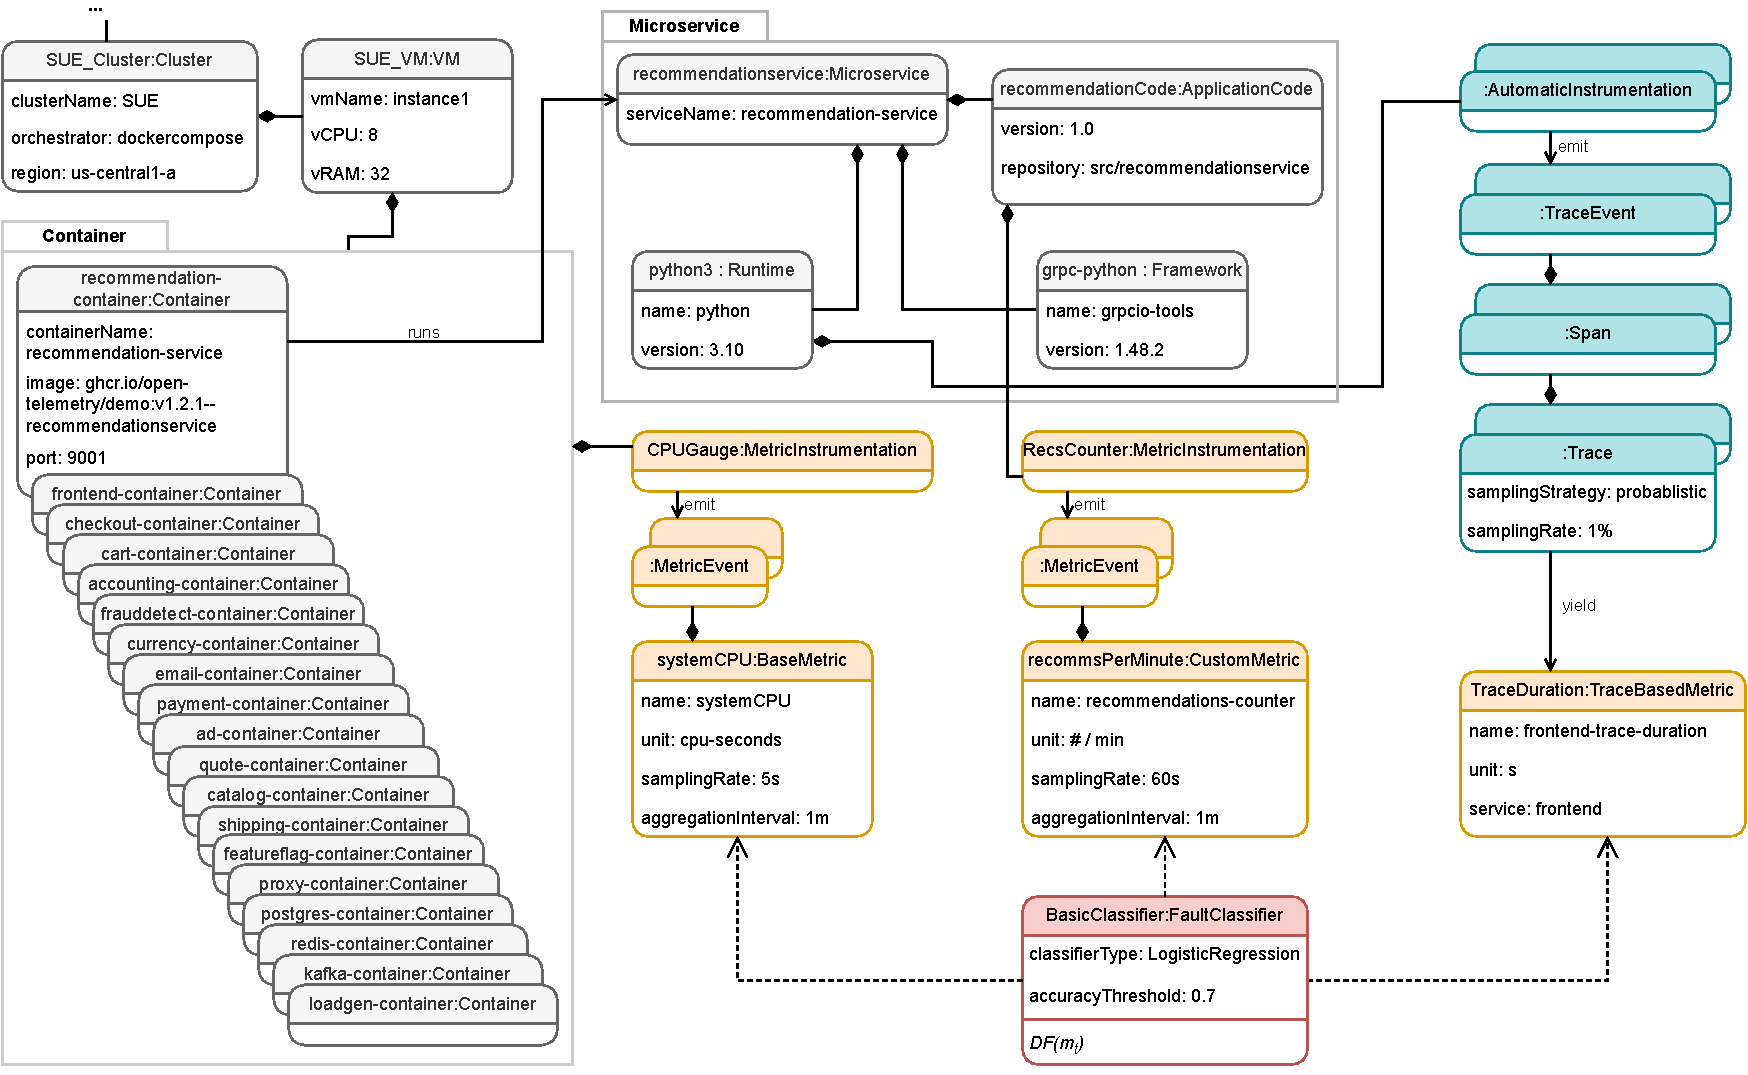
\includegraphics[width=\textwidth]{figures/sue_v3.pdf}
    \caption{SUE with baseline observability configuration}
    \label{fig:sue}
\end{figure*}
Our approach and tooling allows practitioners to evaluate the observability of faults in their microservice application. Besides establishing the effectiveness of the current configuration, they can also use it to reason between observability design alternatives by weighing the observability-cost trade-offs. 
In this section, we demonstrate the applicability our approach by conducting an exemplary evaluation of the observability of a popular open source microservice application. 



\subsection{SUE Setup}
As our system under experiment (SUE), we use the \textit{OpenTelemetry Astronomy Shop Demo}\footnote{\url{https://github.com/open-telemetry/opentelemetry-demo}} microservice application, which is a community project intended to illustrate the use of different observability methods and tools in a near real-world environment. The application consists of 20 core application services plus four dedicated for observability services. We chose this application because it covers a wide range of languages and frameworks across the cloud-native application stack. It is instrumented to collect traces across the whole application, leveraging both automatic and custom instrumentation. Besides traces, it is also instrumented to collect several metrics, including base container health metrics and custom metrics added manually by developers. 
It is a very suitable SUE to showcase OXN, since it offers such a broad spectrum of observability tuning knobs.   

For the experiments, we deploy a fork of the application\footnote{See the \name{} repo for details.} to ensure compatibility with the fault injection functionality of \name{} and to enhance container runtime monitoring. We run \name{} against the SUE on a cloud-based virtual machine (8vCPUs, 32GB Memory). Figure \ref{fig:sue} applies our model for observability design decisions (see \ref{sec:model1}) and shows the snapshot of our SUE at the time of the baseline measurement. We target our experiments on the recommendation service, which mirrors a real-life scenario for developers who, after creating a new service for their application, are faced with instrumentation and configuration decisions to be able to observe this service effectively. 


Our baseline configuration monitors the overall CPU utilization of the system (\texttt{systemCPU}) by collecting and aggregating measurements of the \texttt{CPUGauges} of every container. By default, base metrics are configured with a 5s sampling rate.  Further, the baseline also collects the custom metric \texttt{recommsPerMinute}, through an instrumentation point that the developers added to the recommendation application code. This is configured with a 60s sampling rate by default. For tracing, the application is instrumented with both automatic and custom instrumentation, however the recommendation service in question leverages only automatic instrumentation. The tracing sampling strategy is set to a probabilistic sampler\footnote{\url{https://opentelemetry.io/docs/specs/otel/trace/tracestate-probability-sampling/}} with a 1\% sampling rate.


As a fault detection mechanism, we use the logistic regression classifier that is shipped with \name{} out-of-the-box. Logistic regression is conceptually simple, interpretable,  fast to train on large datasets and
only requires tuning one hyperparameter. %
For training, we split
the experiment data into training and test sets and ensure an equal class balance of fault and non-fault labels via an oversampling technique. %
We further preprocess the telemetry data by z-score normalization. %
After training, we evaluate the classifier's detection function (\textit{\texttt{DF(m\textsubscript{t})}}) on the test data and compute classification accuracy 
with a threshold of $0.7$  as our implementation of $\alpha$ for fault visibility. 

\subsection{Evaluating the Baseline - Results}
We investigate the observability of our SUE with three different types of faults, \texttt{Pause, PacketLoss} and \texttt{NetworkDelay}. For each fault, we run a 10min experiment under constant load (50 concurrent users) and repeat each experiment 10 times.

Figure \ref{fig:plots} plots the metrics we collected over the different experiments with our baseline observability configuration. %
\Cref{tabl:visibilityscores} shows the accuracy of the classifier, averaged over the ten experiment runs, and the resulting fault visibility scores. Because we set our classifier threshold $\alpha$ to 0.7, everything that falls below this threshold will not be identified as fault by our fault detection mechanism, and is therefore invisible.
As we can see, faults like the pause treatment, which simulates an unresponsive service, 
manifest themselves quite prominently across metrics. 
Packet loss is also present in the baseline observability configuration, though with a lower fault coverage (FC) score, since it only manifests in \texttt{systemCPU}. Lastly, faults like delay, which could, for example, simulate a faulty cache, are barely visible in the plots and are not detected by our fault detection mechanism, since the detection function doesn't reach the threshold for any of the collected metrics.

\begin{figure*}[t]
    \centering
    \begin{minipage}{0.52\textwidth}
        \centering
        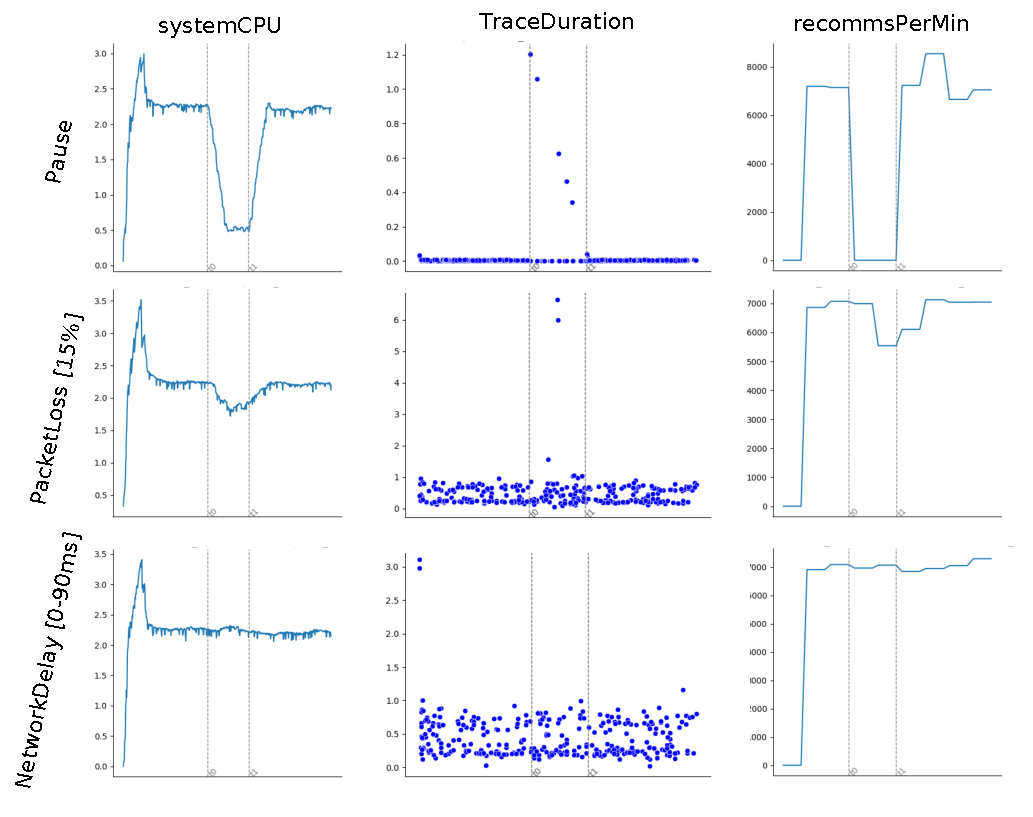
\includegraphics[width=\linewidth]{data/plot_finalversion.pdf}
        \vspace{1em}
        \caption{Experiments run against the SUE using \name{}, showing how different faults appear visually, similar to how a developer would see them in a dashboard. Note how the Pause fault is visible in all metrics. PacketLoss is noticeable in systemCPU but less pronounced in other metrics, with NetworkDelay not being visible at all. In \Cref{fig:plots2}, we see how the changes to the observability configuration proposed in \Cref{fig:alternatives} affect these metrics. }
        \label{fig:plots}
    \end{minipage}%
    \hfill
    \begin{minipage}{0.45\textwidth}
        \centering
        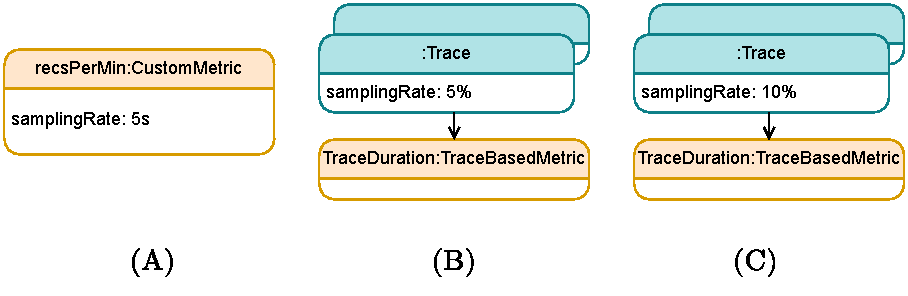
\includegraphics[width=\linewidth]{figures/alternatives_v2.pdf}
        \caption{Observability design alternatives under consideration}
        \label{fig:alternatives}
        \vspace{1em}
        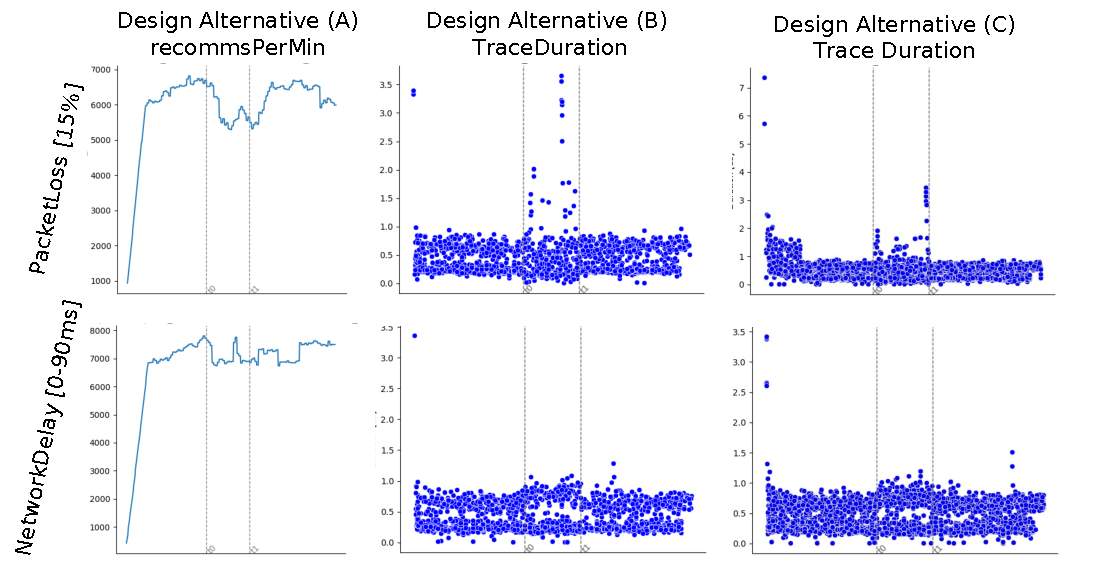
\includegraphics[width=\linewidth]{data/alternative_plots.pdf}
       \caption{Visual changes to fault visibility across design alternatives. Recognize the now more pronounced effect of PacketLoss on \textit{recommsPerMin}, with NetworkDelay still not affecting this metric significantly. NetworkDelay causes a slight noticeable increase in TraceDuration for the longer Traces for both design alternatives B and C.}
        \label{fig:plots2}
    \end{minipage}
\end{figure*}



\begin{table}[h!]
\caption{Fault visibility metrics for default observability configuration} 
\centering
\resizebox{\columnwidth}{!}{
\begin{tabular}{l|lccl}
                      & CPU Util.           & Trace Dur.    & \#Recs/min           & FC         \\ 
\hline
Pause                 & $1 \quad (DF=0.83) $ & $1 \quad (1.00)$ & $1 \quad (0.89)$        & $3/3$      \\
PacketLoss [15\%]     & $1\quad (0.86)$       & $0\quad (0.61)$ & $0\quad (0.42)$        & $1/3$      \\
NetworkDelay [0-90ms] & $0\quad (0.50)$       & $0\quad (0.61)$ & $0\quad (0.43)$        & $0/3$      \\ 
\cline{5-5}
\multicolumn{1}{l}{}  &                     &               & \multicolumn{1}{l}{} & $OFO=2/3$ 
\end{tabular}
}
\label{tabl:visibilityscores}
\end{table}


\subsection{Evaluating Design Alternatives - Results}
To improve the fault observability of our application, we consider three observability design alternatives (see \Cref{fig:alternatives}). The first (Fig. \ref{fig:alternatives}A) is to increase the sampling rate of the application-level recommendation counter, which by default is set to only report once every minute. The other options under consideration are to increase the tracing sampling rate to either 5\% (Fig. \ref{fig:alternatives}B) or 10\% (Fig. \ref{fig:alternatives}C). 

For each observability design alternative, we repeated the  \texttt{PacketLoss} and \texttt{NetworkDelay} experiments, keeping everything else about the SUE and experiment setup the same. 
Figure \ref{fig:plots2} plots the collected metrics after the changes outlined above. \Cref{tab:redesign_results} shows the results regarding fault observability improvements while table  \ref{tabl:configchanges} reveals the costs associated with carrying out each of these observability design decisions (as CPU time [s] summed across the affected services). 

From these results, we can conclude that increasing the interval for the recommendation counter provides better fault coverage for \texttt{PacketLoss} faults, an increase from $1/3$ to $2/3$, but does not affect the $OFO$, since the \texttt{NetworkDelay} fault is still not visible. The second option provides better fault coverage for \texttt{NetworkDelay} faults, an increase from $0/3$ to $1/3$, as well as an increase to the $OFO = 3/3$, now that the delay fault is finally visible. The third option performs similar to the second one in the fault observability metrics. When looking at observability-related trade-offs in the form of cost (see also table \ref{tabl:configchanges}), we see that while B are C viable options to improve $OFO$, B is tied to a lower cost than C, with 3.05\%  overhead instead of 5.33\%. 

Thus, by applying the model, metrics and tooling presented in the paper, we can find a design decision with better fault observability, and we can immediately get a first performance impact assessment. A decision maker can now judge if the higher cost is acceptable and implement the change. Otherwise, more observability experiments can be performed to find a better solution.
Besides that, the model also provides developers and practitioners with a common language to understand, discuss and document their observability design decisions.


\begin{table}[]
    \centering
    \caption{Effects of the Design Alternatives on the fault observability metrics}
    \label{tab:redesign_results}
    \resizebox{\columnwidth}{!}{
        \begin{tabular}{c|ll|cc}
          & PacketLoss [15\%] & NetworkDelay [0-90ms] & $\Delta FC$ & $\Delta OFO$ \\ \hline
        (A) & 1 (DF=0.72)          & 0 (0.59)              & +1          & 0            \\
        (B) & 0 (0.58)          & 1 (0.77)              & +1          & +1           \\
        (C) & 0 (0.60)          & 1 (0.70)               & +1          & +1          
        \end{tabular}
        
    }
    \vspace{1em}
    \caption{Cost of the Design Alternatives in CPU time [s]} \label{tabl:configchanges}
    \centering
    \resizebox{\columnwidth}{!}{
    \begin{tabular}{l|rrrr}
     & Baseline SUE     & (A) & (B) & (C) \\ 
    \hline
    recomm.-service      & 143.30            & 150.74     & 143.86          & 144.63            \\
    otel-col             & 37.38             & 37.49      & 39.05           & 39.99             \\
    prometheus           & 9.01              & 9.07       & 9.07            & 9.48              \\
    jaeger               & 2.14              & 2.17       & 5.70            & 7.96              \\
    \hline
    total                & 191.83 & 199.47     & 197.68          & 202.06            \\ 
    
    overhead             & ~-                & +3.98\%     & +3.05\%          & +5.33\%           
    \end{tabular}
    }
\end{table}






